\begin{example}
    $x^2 + y^2=1$

    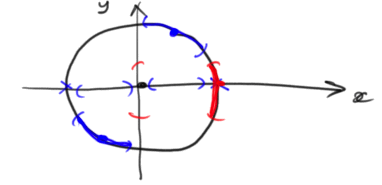
\includegraphics[width=0.3\linewidth]{images/07-06-1.png}

    Нас интересует задание графика функции. Можем сделать это для некоторых точек в некоторых окрестностях, причем где-то мы получим графие $y(x)$, где-то – $x(y)$, а где-то – и то, и то.

    Зависит все от матрицы из производных:

    $f(x, y) = x^2 + y^2 - 1$
    
    $f'(x, y) = (2x, 2y)$

    Посмотрим на какую-то точку: 
    
    $f'(1, 0)= (2, 0)$

    $(2\ 0)\binom{h}{0}\Leftrightarrow h=0$ – выполнено, то есть $x(y)$ есть по аналогии с линейной ситуации.
    
    $(2\ 0)\binom{h}{0}$ – всегда $\Rightarrow$ функция $y(x)$ не получится, нет нужного линейного свойства.

    \textit{Неявная функция} – функции, которые получаются в качестве решения уравнения в окрестности непрерывности (те самые функции, графики которых мы нарисовали).
\end{example}

\begin{theorem}
    \textbf{Теорема о неявной функции.}

    Пусть $D\subset \R^{n+m}$ открытое, $f : D \rightarrow \R^n$ непрерывно дифференцируема, $(\underset{\in \R^n}{a}, \underset{\in \R^m}{b})$ и $f(a, b)=0$, $A := f'(a, b)$ и $A$ удовлетворяет условию: $A(h_0)=0\Rightarrow h_0 =0$. Тогда существует $W$ – окрестность точки $b$ и единственная $g : W\rightarrow \R^n : g(b)=a$, $f(g(y), y)=0\ \forall y\in W$ и эта функция непрерывно дифференцируема.
\end{theorem}
\begin{proof}
    Пусть $F: D \rightarrow \R^{n+m}$, $F(x, y)=(f(x, y), y)$ непрерывно дифференцируема.

    $F'(a, b)= \binom{f'(a, b)}{O \ E}$


    Здесь будет обратимость: $F'(a, b)\binom{h}{k}=\binom{A(h, k)}{k}$, если это $=\binom{0}{0}$, то $k=0$ и $A(h, 0)=0\Rightarrow h=0$, то есть умножение на $F'(a, b)$ –  это инъективное отображение $\Rightarrow F'(a, b)$ обратима. 

    Тогда по теореме об обратной функции $\exists U$ – окрестность $(a, b)$ и $V$ – окрестность $(0, b)$, т.ч. $F: U\rightarrow V$ биекция и $G:=F^{-1}: V \rightarrow U$ непрерывно дифференцируема.

    Как действует эта функция: 

    $G(z, w)=(\varphi(z, w), w)$ (вторая координата должна не меняться)

    $\Rightarrow f(\varphi(z, w), w)=z$

    Возьмем $W$ – окрестность точки $b$, т.ч. $\{0\}\times W\subset V$. Тогда $g: W \rightarrow \R^n$, т.ч. $g(w):=\varphi(0, w)$.

    То, что надо, так как $f(g(w), w)=0$ и $g(b)=a$, $\varphi(0, b)=a$

    Единственность следует из биективности $F$: $f(x, y)=f(\Tilde{x}, y)\Rightarrow F(x, y)=F(\Tilde{x}, y)\overset{\text{$F$ вз. одн.}}{\Rightarrow} (x, y)=(\Tilde{x}, y)\Rightarrow x =\Tilde{x}$
\end{proof}

\subsection{Экстремумы функций}

\begin{definition}
    Пусть $f: E\rightarrow \R$, $a\in E$. 
    
    $a$ – \textit{точка локального минимума}, если $\exists U$-окрестность точки $a$, т.ч. 
    
    $\forall x\in E\cap U$ $f(x)\geq f(a)$.

    $a$ – \textit{точка строгого локального минимума,} если $\exists U$-окрестность точки $a$, т.ч.
    
    $\forall \underset{\neq a}{x}\in E\cap U$ $f(x)> f(a)$.

    $a$ – \textit{точка локального максимума}, если $\exists U$-окрестность точки $a$, т.ч.
    
    $\forall x\in E\cap U$ $f(x)\leq f(a)$.

    $a$ – \textit{точка строгого локального максимума}, если $\exists U$-окрестность точки $a$, т.ч.
    
    $\forall \underset{\neq a}{x}\in E\cap U$ $f(x)> f(a)$.
\end{definition}

\begin{definition}
    Пусть $f: E\rightarrow \R$, $a\in E$. 

    $a$ – \textit{точка экстремума}, если это точка локального минимума или точка локального максимума.

    $a$ – \textit{точка строгого экстремума}, если это точка строгого локального минимума или точка строгого локального максимума.
\end{definition}

\begin{theorem}
    \textbf{Необходимое условие экстремума.}

    Пусть $f: E\rightarrow \R$, $E\subset \R^n$, $a\in \Int E$, $a$ – точка экстремума функции $f$. Тогда если существует $\frac{\partial f}{\partial x_k}(a)$, то $\frac{\partial f}{\partial x_k}(a)=0$. В частности, если $f$ дифференцируема в точке $a$, то $\frac{\partial f}{\partial x_1}(a)=...=\frac{\partial f}{\partial x_n}(a)=0$, то есть $\triangledown f(a)=0$.
\end{theorem}

\begin{proof}
    % picture

    Пусть для определенности $a$ – точка максимума.

    Пусть $g(t) := f(t, a_1, a_2, ..., a_n)$ задана в окрестности точки $a_1$.

    $a_1$ точка локального максимума для функции $g$: $g(a_1)\geq g(t)\ \forall t$ в некоторой окрестности $a_1$.

    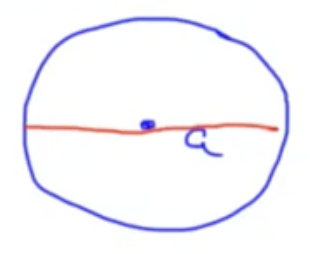
\includegraphics[width=0.1\linewidth]{images/07-06-2.png}

    Если существует $\frac{\partial f}{\partial x_1}(a)$, то $g$ дифференцируема в точке $a_1\Rightarrow g'(a_1)=\frac{\partial f}{\partial x_1}(a)=0$ (необходимое условие для функции от одной переменной).
\end{proof}

\begin{definition}
    $a$ – \textit{стационарная точка функции $f$}, если $\triangledown f(a)=0$.
\end{definition}

\begin{remark}
    Пусть $f$ дважды дифференцируема и $a$ стационарная точка.

    $f(a + h)=f(a)+\frac{1}{2}\sum\limits_{i=1, j=1}^n\frac{\partial^2 f}{\partial x_i \partial x_j}(a) h_i h_j+o(\|h\|^2)$ – \textit{формула Тейлора в стационарной точке}.
\end{remark}

\begin{definition}
    \textit{Квадратичная форма} $Q(h)=\sum\limits_{i, j=1}^n c_{ij}h_ih_j$. Считают, что $c_{ij}=c_{ji}$.

    $C= (c_{ij})^n_{i, j=1}$, $Q(h)=\langle Ch, h\rangle$
\end{definition}

\begin{definition}
    $Q$ – \textit{положительно определенная квадратичная форма}, если $Q(h)\geq 0$ $\forall h\in \R^n$.

    $Q$ – \textit{строго положительно определенная квадратичная форма}, если $Q(h)> 0$ $\forall \underset{\neq 0}{h}\in \R^n$.
\end{definition}

\begin{definition}
    $Q$ – \textit{отрицательно определенная квадратичная форма}, если $Q(h)\leq 0$ $\forall h\in \R^n$.

    $Q$ – \textit{строго отрицательно определенная квадратичная форма}, если $Q(h)< 0$ $\forall \underset{\neq 0}{h}\in \R^n$.
\end{definition}

\begin{lemma}
    Пусть $Q$ строго положительно определенная квадратичная форма. Тогда существует $c>0$, т.ч. $ \forall h\in \R^n$ $Q(h)\geq c\|h\|^2$.
\end{lemma}
\begin{proof}
    $Q(h)=\langle Ch, h\rangle$ – непрерывная функция. 
    
    
    Рассмотрим ее на единичной сфере $S:=\{x\in \R^N\mid \|x\|=1\}$ – компакт $\Rightarrow Q$ достигает наименьшего значения на $S$. Пусть в точке $y\in S: Q(x)\geq Q(y)>0$ $\forall x\in S$.

    Проверим, что $c=Q(y)$ подходит.

    $Q(h)=\langle Ch, h\rangle= \|h\|^2\langle C\frac{h}{\|h\|}, \frac{h}{\|h\|}\rangle$ (вытащили по линейности константу) $\geq \|h\|^2 Q(\frac{h}{\|h\|})$, так как $\frac{h}{\|h\|}\in S$. 

    Если $h=0$, то неравенство очевидно.
\end{proof}

\begin{theorem}
    \textbf{Достаточные условия экстремума.}

    Пусть $f: E\rightarrow \R$, $E\subset \R^n$, $a\in \Int E$, $a$ – стационарная точка, $f$ дважды дифференцируема, $Q(h):=\sum\limits_{i=1, j=1}^n\frac{\partial^2 f}{\partial x_i \partial x_j}(a) h_i h_j$. Тогда:
    \begin{enumerate}
        \item Если $Q$ строго положительно определена, то $a$ точка строгого локального минимума.
        \item Если $Q$ строго отрицательного определена, то $a$ точка строгого локального максимума
        \item Если $a$ точка нестрогого локального минимума, то $Q$ нестрого положительно определена.
        \item Если $a$ точка нестрогого локального максимума, то $Q$ нестрого отрицательно определена.
    \end{enumerate}
\end{theorem}
\begin{proof}
    $f(a+h)=f(a)+\frac{1}{2}\sum\limits_{i=1, j=1}^n\frac{\partial^2 f}{\partial x_i \partial x_j}(a) h_i h_j+o(\|h\|^2)$

    $f(a+h)-f(a)=\frac{1}{2}Q(h)+o(\|h\|^2)$
    \begin{enumerate}
        \item[1.] По лемме $Q(h)\geq c\|h\|^2\Rightarrow f(a+h)-f(a)\geq \frac{c}{2}\|h\|^2 + o(\|h\|^2)=\underbrace{\|h\|^2}_{>0}(\underbrace{\frac{c}{2}+o(1)}_{>0\text{ при $h$ близких к 0}})$ (так как стремится $\frac{c}{2}>0$)
        \item[3.] Зафиксируем $h$: $f(a+th)-f(a)=\frac{1}{2}Q(th)+o(t^2)=t^2\frac{1}{2}Q(h)+o(t^2)$

        $\frac{1}{2}Q(h)\lim\limits_{t\rightarrow 0}\frac{\overbrace{f(a+th)-f(a)}^{\geq 0}}{\underbrace{t^2}_{> 0}}\geq 0 \Rightarrow Q(h)\geq 0 $
    \end{enumerate}
\end{proof}

\begin{example}
    $f(x, y)=x^4 + y^4 - 36xy$

    $\begin{array}{lll}
        \frac{\partial f}{\partial x}=4x^3 - 36y &  \frac{\partial f}{\partial y}=4y^3 - 36x & \frac{\partial f}{\partial x}=\frac{\partial f}{\partial y}=0
    \end{array}$

    $\left\{\begin{array}{lll}
         x^3=9y & y = \frac{x^3}{9} & \\
         y^3=9x & 9x=y^3=(\frac{x^3}{9})^3 & x^9=3^8x
    \end{array}\right.\Rightarrow \left[\begin{array}{l}
         x=0  \\
         x=\pm 3 
    \end{array}\right.\Rightarrow (0, 0)$, $(3, 3)$, $(-3, -3)$ удовлетворяют необходимому условию эксттремума.

    $\begin{array}{llll}
       \frac{\partial^2 f}{\partial x^2}=12x^2  & \frac{\partial^2 f}{\partial y^2}=12y^2 & \frac{\partial^2 f}{\partial x\partial y}=-36 &
       \begin{pmatrix}
           12x^2 & -36 \\
           -36 & 12y^2
       \end{pmatrix}
    \end{array}$

    $\begin{pmatrix}
           x^2 & -3 \\
           -3 & y^2
     \end{pmatrix}$

    \begin{enumerate}
        \item $\begin{array}{lll}
             (0, 0) & \begin{pmatrix}
                   0 & -3 \\
                   -3 & 0
             \end{pmatrix} & 
             \det \begin{pmatrix}
                   0 & -3 \\
                   -3 & 0
             \end{pmatrix} = -9 < 0
                \end{array}$
                
        Нет знакоопределенности $\Rightarrow$ не точка экстремума.
        \item $\begin{array}{lll}
             (3, 3) \text{ и } (-3, -3)& \begin{pmatrix}
                   9 & -3 \\
                   -3 & 9
             \end{pmatrix} & 
             \det \begin{pmatrix}
                   9 & -3 \\
                   -3 & 9
             \end{pmatrix} = 81-9 > 0
                \end{array}$

        Положительно определена $\Rightarrow$ точка строгого локального минимума.
    \end{enumerate}
\end{example}
    
\begin{statement}
    \textbf{Критерий Сильвестра.}

    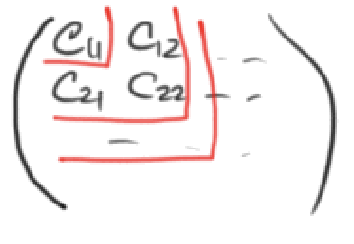
\includegraphics[width=0.2\linewidth]{images/07-06-3.png}

    \begin{enumerate}
        \item $c_{11} > 0$

            $\det \begin{pmatrix}
                   c_{11} & c_{12} \\
                   c_{21} & c_{22}
             \end{pmatrix}>0$

             $\det \begin{pmatrix}
                   c_{11} & c_{12} & c_{13} \\
                   c_{21} & c_{22} & c_{23} \\
                   c_{31} & c_{32} & c_{33}
             \end{pmatrix}>0$

             ...

             $\Leftrightarrow$ строгая положительная определенность.
        \item $c_{11} < 0$

            $\det \begin{pmatrix}
                   c_{11} & c_{12} \\
                   c_{21} & c_{22}
             \end{pmatrix}<0$

             $\det \begin{pmatrix}
                   c_{11} & c_{12} & c_{13} \\
                   c_{21} & c_{22} & c_{23} \\
                   c_{31} & c_{32} & c_{33}
             \end{pmatrix}<0$

             ...

             $\Leftrightarrow$ строгая отрицательная определенность.
    \end{enumerate}
\end{statement}

\begin{definition}
    Пусть $f: D\rightarrow \R$, $D\subset \R^{n+m}$ открытое, $\Phi: D\rightarrow \R^m$, $a\in D$, $\Phi(a) =0$. Тогда:
    \begin{enumerate}
        \item $a$ точка \textit{условного локального минимума при условии $\Phi(x) = 0$}, если $\exists U$ – окрестность точки $a$, т.ч. $\forall x\in U$, удовлетворяющего условию $\Phi(x)=0$, $f(x)\geq f(a)$.
        \item $a$ \textit{точка строго условного локального минимума при условии $\Phi(x) = 0$}, если $\exists U$ – окрестность точки $a$, т.ч. $\forall \underset{\neq a}{x}\in U$, удовлетворяющего условию $\Phi(x)=0$, $f(x)>f(a)$.
    \end{enumerate}
\end{definition}

\begin{theorem}
    \textbf{Метод неопределенных множителей Лагранжа}
    
    Пусть $f: D \rightarrow \R$ непрерывно дифференцируема,  $\Phi: D \rightarrow \R^m$ непрерывно дифференцируема, $a\in D$, $\Phi(a) =0$, $D$ открытое. 

    Если $a$ точка условного экстремума (при условии $\Phi(x) = 0$), то $\triangledown f_{(a)}$, $\triangledown \Phi_1^{(a)}$, ..., $\triangledown \Phi_m^{(a)}$ линейно зависимы.
\end{theorem}

\begin{remark}~
    \begin{enumerate}
        \item Пусть $\triangledown \Phi_1(a)$, ...,  $\triangledown \Phi_m(a)$ линейно независимы. Тогда $\triangledown f(a) =\lambda_1 \Phi_1(a)  + ... + \lambda_m\triangledown \Phi_m(a)$.

        Эти $\lambda_i$ – \textit{неопределенные коэффициенты Лагранжа}.
        \item Что значит линейная независимость $\triangledown \Phi_1(a)$, ...,  $\triangledown \Phi_m(a)$? Это строки матрицы $\Phi'(a)$, то есть ранг матрицы $\Phi'(a)$ максимально возможный.

    \end{enumerate}
\end{remark}

Хотим доказать, что если ранг $\Phi'(a)$ максимально возможный, $a$ точка условного экстремума, то  $\triangledown f(a) =\lambda_1 \Phi_1(a)  + ... + \lambda_m\triangledown \Phi_m(a)$ для некоторых $\lambda_1, ..., \lambda_m\in \R$.

\begin{proof}
    Пусть минор по последним столбцам у $\Phi'(a)$ невырожденный:

    $\Phi'(a)(0, h)=0\Rightarrow h=0$

    $a=(b, c)$. Тогда по теореме о неявной функции $\exists W$ окрестность точки $b$, $g: W\rightarrow \R^n$ непрерывно дифференцируема, т.ч. $\Phi(x, g(x))=0\ \forall x\in W$.

    Рассмотрим функцию $\underbrace{h(x)}_{\leq h(b)=f(b, g(b))= }:=\underbrace{f(x, g(x))}_{\leq f(a)}$. Тогда $b$ – локальный экстремум функции $h$ (для определенности рассматриваем условный максимум).

    Тогда по необходимому условию экстремума $h'(b)$ – нулевая матрица.

    $h$ – композиция $f$ и $x\mapsto \binom{x}{g(x)}$. $0=h'(b)=f'(a)\binom{E}{g'(b)}=(f_x'(a)f_y'(a))\binom{E}{g'(b)}=f_x'(a)+f'_y(a)g'(b)$ строка

    $\Phi(x, g(x))\equiv 0\Rightarrow \Phi'_x(a)+\Phi'_y(a)g'(b)=0$ матрица

    Возьмем $\lambda =(\lambda_1, \lambda_2, ..., \lambda_m)$. 
    
    $\lambda \Phi'_x(a)+\lambda\Phi'_y(a)g'(b)=0\Rightarrow\underbrace{(f'_x(a) - \lambda \Phi'_x(a))}_{=0}+\underbrace{(f'_y(a)-\lambda\Phi'_y(a))}_{=0}g'(b)=0$

    Нужно так подобрать $\lambda$, что $f'_y(a)-\lambda \Phi'_y(a)=0\Rightarrow\lambda \Phi'_y(a)=f'_y(a)$
\end{proof}

\begin{definition}
    $f-\lambda \Phi=f-\lambda_1 \Phi_1 - ... \lambda_m \Phi_m$ –  \textit{функция Лагранжа}.
\end{definition}

\begin{remark}
    Условие из метода множителей Лагранжа можно записать так: $\triangledown (f-\lambda \Phi)(a)=0$.
\end{remark}

\begin{example}
    Наибольшее и наименьшее значение квадратичной формы на сферей

    $A$ – симметричная матрица, $Q(x)=\langle Ax, x\rangle$, $\|x\|^2=1$

    $F(x)=Q(x)=\lambda (\|x\|^2-1)=\sum\limits_{i, j=1}^n a_{ij}x_ix_j-\lambda =\sum\limits_{i=1}^nx_i^2+\lambda$

    В точках условного экстремума $\triangledown F=0$.

    $m=1$: $\Phi(x) =\sum\limits_{i=1}^n x_i^2 -1$, $\Phi'(x)=(2x_1, 2x_2, ..., 2x_n)$

    $\frac{\partial f}{\partial x_k}(x)=\sum\limits_{i=1}^n a_{ik}x_i+\sum\limits_{j=1}^n a_{kj}x_j-\lambda \cdot 2x_k =2\sum\limits_{i=1}^n a_{ik}x_i-2\lambda x_k=0\Rightarrow \lambda$ –  собственное число матрицы, $x_k$ – соответствующий единичный собственный вектор

    $Q(x)=\langle Ax, x \rangle =\langle \lambda x, x\rangle=\lambda\langle  x, x\rangle =\lambda$
\end{example}

\begin{theorem}
    Наибольшее (наименьшее) значение квадратичной формы $Q(h)=\langle Ah, h\rangle$ ($A$ – симметричная матрица) на единичной сфере – это наибольшее (наименьшее) собственное число матрицы. Они достигаются на соответствующих единичных собственных векторах.
\end{theorem}
\begin{corollary}
    $\|A\|=\max \{\sqrt{\lambda}\mid \lambda \text{ – собственное число матрицы }A^TA\}$
\end{corollary}
\begin{proof}
    $\|A\|^2=\max\limits_{\|x\|=1}\|Ax\|^2 =\max\limits_{\|x\|=1} \langle Ax, Ax\rangle= \max\limits_{\|x\|=1}\langle A^TAx, x\rangle$
\end{proof}